\documentclass[1p]{elsarticle_modified}
%\bibliographystyle{elsarticle-num}

%\usepackage[colorlinks]{hyperref}
%\usepackage{abbrmath_seonhwa} %\Abb, \Ascr, \Acal ,\Abf, \Afrak
\usepackage{amsfonts}
\usepackage{amssymb}
\usepackage{amsmath}
\usepackage{amsthm}
\usepackage{scalefnt}
\usepackage{amsbsy}
\usepackage{kotex}
\usepackage{caption}
\usepackage{subfig}
\usepackage{color}
\usepackage{graphicx}
\usepackage{xcolor} %% white, black, red, green, blue, cyan, magenta, yellow
\usepackage{float}
\usepackage{setspace}
\usepackage{hyperref}

\usepackage{tikz}
\usetikzlibrary{arrows}

\usepackage{multirow}
\usepackage{array} % fixed length table
\usepackage{hhline}

%%%%%%%%%%%%%%%%%%%%%
\makeatletter
\renewcommand*\env@matrix[1][\arraystretch]{%
	\edef\arraystretch{#1}%
	\hskip -\arraycolsep
	\let\@ifnextchar\new@ifnextchar
	\array{*\c@MaxMatrixCols c}}
\makeatother %https://tex.stackexchange.com/questions/14071/how-can-i-increase-the-line-spacing-in-a-matrix
%%%%%%%%%%%%%%%

\usepackage[normalem]{ulem}

\newcommand{\msout}[1]{\ifmmode\text{\sout{\ensuremath{#1}}}\else\sout{#1}\fi}
%SOURCE: \msout is \stkout macro in https://tex.stackexchange.com/questions/20609/strikeout-in-math-mode

\newcommand{\cancel}[1]{
	\ifmmode
	{\color{red}\msout{#1}}
	\else
	{\color{red}\sout{#1}}
	\fi
}

\newcommand{\add}[1]{
	{\color{blue}\uwave{#1}}
}

\newcommand{\replace}[2]{
	\ifmmode
	{\color{red}\msout{#1}}{\color{blue}\uwave{#2}}
	\else
	{\color{red}\sout{#1}}{\color{blue}\uwave{#2}}
	\fi
}

\newcommand{\Sol}{\mathcal{S}} %segment
\newcommand{\D}{D} %diagram
\newcommand{\A}{\mathcal{A}} %arc


%%%%%%%%%%%%%%%%%%%%%%%%%%%%%5 test

\def\sl{\operatorname{\textup{SL}}(2,\Cbb)}
\def\psl{\operatorname{\textup{PSL}}(2,\Cbb)}
\def\quan{\mkern 1mu \triangleright \mkern 1mu}

\theoremstyle{definition}
\newtheorem{thm}{Theorem}[section]
\newtheorem{prop}[thm]{Proposition}
\newtheorem{lem}[thm]{Lemma}
\newtheorem{ques}[thm]{Question}
\newtheorem{cor}[thm]{Corollary}
\newtheorem{defn}[thm]{Definition}
\newtheorem{exam}[thm]{Example}
\newtheorem{rmk}[thm]{Remark}
\newtheorem{alg}[thm]{Algorithm}

\newcommand{\I}{\sqrt{-1}}
\begin{document}

%\begin{frontmatter}
%
%\title{Boundary parabolic representations of knots up to 8 crossings}
%
%%% Group authors per affiliation:
%\author{Yunhi Cho} 
%\address{Department of Mathematics, University of Seoul, Seoul, Korea}
%\ead{yhcho@uos.ac.kr}
%
%
%\author{Seonhwa Kim} %\fnref{s_kim}}
%\address{Center for Geometry and Physics, Institute for Basic Science, Pohang, 37673, Korea}
%\ead{ryeona17@ibs.re.kr}
%
%\author{Hyuk Kim}
%\address{Department of Mathematical Sciences, Seoul National University, Seoul 08826, Korea}
%\ead{hyukkim@snu.ac.kr}
%
%\author{Seokbeom Yoon}
%\address{Department of Mathematical Sciences, Seoul National University, Seoul, 08826,  Korea}
%\ead{sbyoon15@snu.ac.kr}
%
%\begin{abstract}
%We find all boundary parabolic representation of knots up to 8 crossings.
%
%\end{abstract}
%\begin{keyword}
%    \MSC[2010] 57M25 
%\end{keyword}
%
%\end{frontmatter}

%\linenumbers
%\tableofcontents
%
\newcommand\colored[1]{\textcolor{white}{\rule[-0.35ex]{0.8em}{1.4ex}}\kern-0.8em\color{red} #1}%
%\newcommand\colored[1]{\textcolor{white}{ #1}\kern-2.17ex	\textcolor{white}{ #1}\kern-1.81ex	\textcolor{white}{ #1}\kern-2.15ex\color{red}#1	}

{\Large $\underline{11a_{82}~(K11a_{82})}$}

\setlength{\tabcolsep}{10pt}
\renewcommand{\arraystretch}{1.6}
\vspace{1cm}\begin{tabular}{m{100pt}>{\centering\arraybackslash}m{274pt}}
\multirow{5}{120pt}{
	\centering
	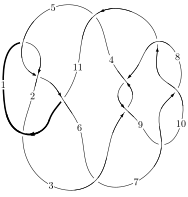
\includegraphics[width=112pt]{../../../GIT/diagram.site/Diagrams/png/331_11a_82.png}\\
\ \ \ A knot diagram\footnotemark}&
\allowdisplaybreaks
\textbf{Linearized knot diagam} \\
\cline{2-2}
 &
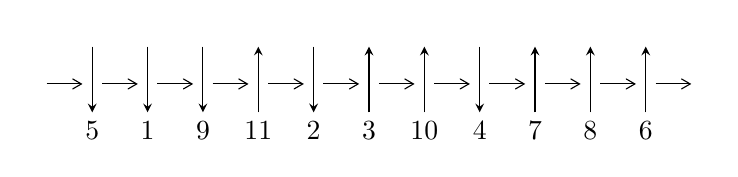
\begin{tikzpicture}[x=20pt, y=17pt]
	% nodes
	\node (C0) at (0, 0) {};
	\node (C1) at (1, 0) {};
	\node (C1U) at (1, +1) {};
	\node (C1D) at (1, -1) {5};

	\node (C2) at (2, 0) {};
	\node (C2U) at (2, +1) {};
	\node (C2D) at (2, -1) {1};

	\node (C3) at (3, 0) {};
	\node (C3U) at (3, +1) {};
	\node (C3D) at (3, -1) {9};

	\node (C4) at (4, 0) {};
	\node (C4U) at (4, +1) {};
	\node (C4D) at (4, -1) {11};

	\node (C5) at (5, 0) {};
	\node (C5U) at (5, +1) {};
	\node (C5D) at (5, -1) {2};

	\node (C6) at (6, 0) {};
	\node (C6U) at (6, +1) {};
	\node (C6D) at (6, -1) {3};

	\node (C7) at (7, 0) {};
	\node (C7U) at (7, +1) {};
	\node (C7D) at (7, -1) {10};

	\node (C8) at (8, 0) {};
	\node (C8U) at (8, +1) {};
	\node (C8D) at (8, -1) {4};

	\node (C9) at (9, 0) {};
	\node (C9U) at (9, +1) {};
	\node (C9D) at (9, -1) {7};

	\node (C10) at (10, 0) {};
	\node (C10U) at (10, +1) {};
	\node (C10D) at (10, -1) {8};

	\node (C11) at (11, 0) {};
	\node (C11U) at (11, +1) {};
	\node (C11D) at (11, -1) {6};
	\node (C12) at (12, 0) {};

	% arrows
	\draw[->,>={angle 60}]
	(C0) edge (C1) (C1) edge (C2) (C2) edge (C3) (C3) edge (C4) (C4) edge (C5) (C5) edge (C6) (C6) edge (C7) (C7) edge (C8) (C8) edge (C9) (C9) edge (C10) (C10) edge (C11) (C11) edge (C12) ;	\draw[->,>=stealth]
	(C1U) edge (C1D) (C2U) edge (C2D) (C3U) edge (C3D) (C4D) edge (C4U) (C5U) edge (C5D) (C6D) edge (C6U) (C7D) edge (C7U) (C8U) edge (C8D) (C9D) edge (C9U) (C10D) edge (C10U) (C11D) edge (C11U) ;
	\end{tikzpicture} \\
\hhline{~~} \\& 
\textbf{Solving Sequence} \\ \cline{2-2} 
 &
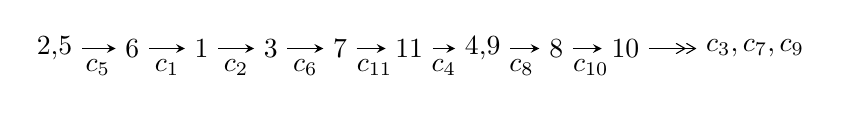
\begin{tikzpicture}[x=25pt, y=7pt]
	% node
	\node (A0) at (-1/8, 0) {2,5};
	\node (A1) at (1, 0) {6};
	\node (A2) at (2, 0) {1};
	\node (A3) at (3, 0) {3};
	\node (A4) at (4, 0) {7};
	\node (A5) at (5, 0) {11};
	\node (A6) at (97/16, 0) {4,9};
	\node (A7) at (57/8, 0) {8};
	\node (A8) at (65/8, 0) {10};
	\node (C1) at (1/2, -1) {$c_{5}$};
	\node (C2) at (3/2, -1) {$c_{1}$};
	\node (C3) at (5/2, -1) {$c_{2}$};
	\node (C4) at (7/2, -1) {$c_{6}$};
	\node (C5) at (9/2, -1) {$c_{11}$};
	\node (C6) at (11/2, -1) {$c_{4}$};
	\node (C7) at (53/8, -1) {$c_{8}$};
	\node (C8) at (61/8, -1) {$c_{10}$};
	\node (A9) at (10, 0) {$c_{3},c_{7},c_{9}$};

	% edge
	\draw[->,>=stealth]	
	(A0) edge (A1) (A1) edge (A2) (A2) edge (A3) (A3) edge (A4) (A4) edge (A5) (A5) edge (A6) (A6) edge (A7) (A7) edge (A8) ;
	\draw[->>,>={angle 60}]	
	(A8) edge (A9);
\end{tikzpicture} \\ 

\end{tabular} \\

\footnotetext{
The image of knot diagram is generated by the software ``\textbf{Draw programme}" developed by Andrew Bartholomew(\url{http://www.layer8.co.uk/maths/draw/index.htm\#Running-draw}), where we modified some parts for our purpose(\url{https://github.com/CATsTAILs/LinksPainter}).
}\phantom \\ \newline 
\centering \textbf{Ideals for irreducible components\footnotemark of $X_{\text{par}}$} 
 
\begin{align*}
I^u_{1}&=\langle 
2 u^{52}+4 u^{51}+\cdots+b+2,\;2 u^{52}+2 u^{51}+\cdots+a+1,\;u^{53}+2 u^{52}+\cdots+u+1\rangle \\
I^u_{2}&=\langle 
u^5- u^3+b+u,\;u^4- u^2+a+u,\;u^6- u^5- u^4+2 u^3- u+1\rangle \\
\\
\end{align*}
\raggedright * 2 irreducible components of $\dim_{\mathbb{C}}=0$, with total 59 representations.\\
\footnotetext{All coefficients of polynomials are rational numbers. But the coefficients are sometimes approximated in decimal forms when there is not enough margin.}
\newpage
\renewcommand{\arraystretch}{1}
\centering \section*{I. $I^u_{1}= \langle 2 u^{52}+4 u^{51}+\cdots+b+2,\;2 u^{52}+2 u^{51}+\cdots+a+1,\;u^{53}+2 u^{52}+\cdots+u+1 \rangle$}
\flushleft \textbf{(i) Arc colorings}\\
\begin{tabular}{m{7pt} m{180pt} m{7pt} m{180pt} }
\flushright $a_{2}=$&$\begin{pmatrix}0\\u\end{pmatrix}$ \\
\flushright $a_{5}=$&$\begin{pmatrix}1\\0\end{pmatrix}$ \\
\flushright $a_{6}=$&$\begin{pmatrix}1\\u^2\end{pmatrix}$ \\
\flushright $a_{1}=$&$\begin{pmatrix}u\\u\end{pmatrix}$ \\
\flushright $a_{3}=$&$\begin{pmatrix}- u^3\\- u^3+u\end{pmatrix}$ \\
\flushright $a_{7}=$&$\begin{pmatrix}u^8- u^6+u^4+1\\u^8-2 u^6+2 u^4\end{pmatrix}$ \\
\flushright $a_{11}=$&$\begin{pmatrix}u^3\\u^5- u^3+u\end{pmatrix}$ \\
\flushright $a_{4}=$&$\begin{pmatrix}u^8- u^6+u^4+1\\u^{10}-2 u^8+3 u^6-2 u^4+u^2\end{pmatrix}$ \\
\flushright $a_{9}=$&$\begin{pmatrix}-2 u^{52}-2 u^{51}+\cdots-3 u-1\\-2 u^{52}-4 u^{51}+\cdots-2 u-2\end{pmatrix}$ \\
\flushright $a_{8}=$&$\begin{pmatrix}u^{50}+u^{49}+\cdots+2 u^2-3 u\\- u^{31}+7 u^{29}+\cdots+2 u^2- u\end{pmatrix}$ \\
\flushright $a_{10}=$&$\begin{pmatrix}- u^{52}- u^{51}+\cdots+3 u^2-3 u\\- u^{52}-2 u^{51}+\cdots- u-1\end{pmatrix}$\\ \flushright $a_{10}=$&$\begin{pmatrix}- u^{52}- u^{51}+\cdots+3 u^2-3 u\\- u^{52}-2 u^{51}+\cdots- u-1\end{pmatrix}$\\&\end{tabular}
\flushleft \textbf{(ii) Obstruction class $= -1$}\\~\\
\flushleft \textbf{(iii) Cusp Shapes $= -4 u^{52}-6 u^{51}+\cdots+9 u^2-2$}\\~\\
\newpage\renewcommand{\arraystretch}{1}
\flushleft \textbf{(iv) u-Polynomials at the component}\newline \\
\begin{tabular}{m{50pt}|m{274pt}}
Crossings & \hspace{64pt}u-Polynomials at each crossing \\
\hline $$\begin{aligned}c_{1},c_{5}\end{aligned}$$&$\begin{aligned}
&u^{53}+2 u^{52}+\cdots+u+1
\end{aligned}$\\
\hline $$\begin{aligned}c_{2}\end{aligned}$$&$\begin{aligned}
&u^{53}+24 u^{52}+\cdots+5 u+1
\end{aligned}$\\
\hline $$\begin{aligned}c_{3},c_{8}\end{aligned}$$&$\begin{aligned}
&u^{53}- u^{52}+\cdots-64 u-64
\end{aligned}$\\
\hline $$\begin{aligned}c_{4},c_{6}\end{aligned}$$&$\begin{aligned}
&u^{53}-2 u^{52}+\cdots-144 u+36
\end{aligned}$\\
\hline $$\begin{aligned}c_{7},c_{9},c_{10}\end{aligned}$$&$\begin{aligned}
&u^{53}+7 u^{52}+\cdots-6 u-1
\end{aligned}$\\
\hline $$\begin{aligned}c_{11}\end{aligned}$$&$\begin{aligned}
&u^{53}+6 u^{52}+\cdots-5 u-1
\end{aligned}$\\
\hline
\end{tabular}\\~\\
\newpage\renewcommand{\arraystretch}{1}
\flushleft \textbf{(v) Riley Polynomials at the component}\newline \\
\begin{tabular}{m{50pt}|m{274pt}}
Crossings & \hspace{64pt}Riley Polynomials at each crossing \\
\hline $$\begin{aligned}c_{1},c_{5}\end{aligned}$$&$\begin{aligned}
&y^{53}-24 y^{52}+\cdots+5 y-1
\end{aligned}$\\
\hline $$\begin{aligned}c_{2}\end{aligned}$$&$\begin{aligned}
&y^{53}+12 y^{52}+\cdots-27 y-1
\end{aligned}$\\
\hline $$\begin{aligned}c_{3},c_{8}\end{aligned}$$&$\begin{aligned}
&y^{53}+39 y^{52}+\cdots+8192 y-4096
\end{aligned}$\\
\hline $$\begin{aligned}c_{4},c_{6}\end{aligned}$$&$\begin{aligned}
&y^{53}-48 y^{52}+\cdots+10728 y-1296
\end{aligned}$\\
\hline $$\begin{aligned}c_{7},c_{9},c_{10}\end{aligned}$$&$\begin{aligned}
&y^{53}-55 y^{52}+\cdots+14 y-1
\end{aligned}$\\
\hline $$\begin{aligned}c_{11}\end{aligned}$$&$\begin{aligned}
&y^{53}+54 y^{51}+\cdots+45 y-1
\end{aligned}$\\
\hline
\end{tabular}\\~\\
\newpage\flushleft \textbf{(vi) Complex Volumes and Cusp Shapes}
$$\begin{array}{c|c|c}  
\text{Solutions to }I^u_{1}& \I (\text{vol} + \sqrt{-1}CS) & \text{Cusp shape}\\
 \hline 
\begin{aligned}
u &= -0.974772 + 0.241666 I \\
a &= -0.636930 - 0.032053 I \\
b &= -0.591584 + 0.107088 I\end{aligned}
 & -1.72966 + 0.52144 I & -5.77451 - 0.49909 I \\ \hline\begin{aligned}
u &= -0.974772 - 0.241666 I \\
a &= -0.636930 + 0.032053 I \\
b &= -0.591584 - 0.107088 I\end{aligned}
 & -1.72966 - 0.52144 I & -5.77451 + 0.49909 I \\ \hline\begin{aligned}
u &= \phantom{-}0.799486 + 0.620081 I \\
a &= \phantom{-}0.938129 - 0.652027 I \\
b &= \phantom{-}0.075820 + 0.997850 I\end{aligned}
 & \phantom{-}8.47576 - 2.42942 I & \phantom{-}9.05009 + 3.27749 I \\ \hline\begin{aligned}
u &= \phantom{-}0.799486 - 0.620081 I \\
a &= \phantom{-}0.938129 + 0.652027 I \\
b &= \phantom{-}0.075820 - 0.997850 I\end{aligned}
 & \phantom{-}8.47576 + 2.42942 I & \phantom{-}9.05009 - 3.27749 I \\ \hline\begin{aligned}
u &= -0.547871 + 0.781328 I \\
a &= -0.308221 - 0.327517 I \\
b &= -0.62380 - 2.01056 I\end{aligned}
 & \phantom{-}13.9720 + 5.2869 I & \phantom{-}9.56069 - 3.45269 I \\ \hline\begin{aligned}
u &= -0.547871 - 0.781328 I \\
a &= -0.308221 + 0.327517 I \\
b &= -0.62380 + 2.01056 I\end{aligned}
 & \phantom{-}13.9720 - 5.2869 I & \phantom{-}9.56069 + 3.45269 I \\ \hline\begin{aligned}
u &= \phantom{-}0.972428 + 0.431066 I \\
a &= -1.87141 + 0.12673 I \\
b &= -0.202339 - 1.299480 I\end{aligned}
 & \phantom{-}0.32639 - 1.89843 I & \phantom{-}4.06618 + 4.82062 I \\ \hline\begin{aligned}
u &= \phantom{-}0.972428 - 0.431066 I \\
a &= -1.87141 - 0.12673 I \\
b &= -0.202339 + 1.299480 I\end{aligned}
 & \phantom{-}0.32639 + 1.89843 I & \phantom{-}4.06618 - 4.82062 I \\ \hline\begin{aligned}
u &= -1.06609\phantom{ +0.000000I} \\
a &= \phantom{-}1.05441\phantom{ +0.000000I} \\
b &= \phantom{-}1.12898\phantom{ +0.000000I}\end{aligned}
 & \phantom{-}3.31477\phantom{ +0.000000I} & \phantom{-}2.11820\phantom{ +0.000000I} \\ \hline\begin{aligned}
u &= \phantom{-}1.068650 + 0.060095 I \\
a &= -0.00519 - 3.08536 I \\
b &= \phantom{-}0.33759 - 1.38633 I\end{aligned}
 & \phantom{-}1.15819 + 2.52423 I & \phantom{-}1.16527 - 3.38233 I\\
 \hline 
 \end{array}$$\newpage$$\begin{array}{c|c|c}  
\text{Solutions to }I^u_{1}& \I (\text{vol} + \sqrt{-1}CS) & \text{Cusp shape}\\
 \hline 
\begin{aligned}
u &= \phantom{-}1.068650 - 0.060095 I \\
a &= -0.00519 + 3.08536 I \\
b &= \phantom{-}0.33759 + 1.38633 I\end{aligned}
 & \phantom{-}1.15819 - 2.52423 I & \phantom{-}1.16527 + 3.38233 I \\ \hline\begin{aligned}
u &= -0.436206 + 0.813289 I \\
a &= -0.314398 + 0.221559 I \\
b &= \phantom{-}0.30278 + 2.64405 I\end{aligned}
 & \phantom{-}13.3377 - 8.5290 I & \phantom{-}8.89957 + 3.73071 I \\ \hline\begin{aligned}
u &= -0.436206 - 0.813289 I \\
a &= -0.314398 - 0.221559 I \\
b &= \phantom{-}0.30278 - 2.64405 I\end{aligned}
 & \phantom{-}13.3377 + 8.5290 I & \phantom{-}8.89957 - 3.73071 I \\ \hline\begin{aligned}
u &= \phantom{-}0.480967 + 0.776724 I \\
a &= \phantom{-}0.649586 - 0.094929 I \\
b &= -0.658204 + 0.307267 I\end{aligned}
 & \phantom{-}8.70701 + 1.51183 I & \phantom{-}8.31702 - 0.27451 I \\ \hline\begin{aligned}
u &= \phantom{-}0.480967 - 0.776724 I \\
a &= \phantom{-}0.649586 + 0.094929 I \\
b &= -0.658204 - 0.307267 I\end{aligned}
 & \phantom{-}8.70701 - 1.51183 I & \phantom{-}8.31702 + 0.27451 I \\ \hline\begin{aligned}
u &= -0.500888 + 0.763334 I \\
a &= \phantom{-}0.092905 + 0.528334 I \\
b &= \phantom{-}0.80992 + 2.38721 I\end{aligned}
 & \phantom{-}6.63504 + 1.32263 I & \phantom{-}7.88405 - 2.69846 I \\ \hline\begin{aligned}
u &= -0.500888 - 0.763334 I \\
a &= \phantom{-}0.092905 - 0.528334 I \\
b &= \phantom{-}0.80992 - 2.38721 I\end{aligned}
 & \phantom{-}6.63504 - 1.32263 I & \phantom{-}7.88405 + 2.69846 I \\ \hline\begin{aligned}
u &= -0.458619 + 0.779636 I \\
a &= \phantom{-}0.215540 - 0.450057 I \\
b &= -0.54372 - 2.68876 I\end{aligned}
 & \phantom{-}6.39750 - 4.28616 I & \phantom{-}7.23871 + 3.29000 I \\ \hline\begin{aligned}
u &= -0.458619 - 0.779636 I \\
a &= \phantom{-}0.215540 + 0.450057 I \\
b &= -0.54372 + 2.68876 I\end{aligned}
 & \phantom{-}6.39750 + 4.28616 I & \phantom{-}7.23871 - 3.29000 I \\ \hline\begin{aligned}
u &= -1.038310 + 0.379912 I \\
a &= \phantom{-}0.000675 + 1.082270 I \\
b &= \phantom{-}0.397647 + 0.928057 I\end{aligned}
 & -2.65480 + 1.42970 I & -5.16065 - 0.45006 I\\
 \hline 
 \end{array}$$\newpage$$\begin{array}{c|c|c}  
\text{Solutions to }I^u_{1}& \I (\text{vol} + \sqrt{-1}CS) & \text{Cusp shape}\\
 \hline 
\begin{aligned}
u &= -1.038310 - 0.379912 I \\
a &= \phantom{-}0.000675 - 1.082270 I \\
b &= \phantom{-}0.397647 - 0.928057 I\end{aligned}
 & -2.65480 - 1.42970 I & -5.16065 + 0.45006 I \\ \hline\begin{aligned}
u &= -1.015080 + 0.482408 I \\
a &= -0.90550 - 1.83401 I \\
b &= -1.37700 - 0.93578 I\end{aligned}
 & \phantom{-}0.80550 + 3.99450 I & \phantom{-}2.19146 - 3.84882 I \\ \hline\begin{aligned}
u &= -1.015080 - 0.482408 I \\
a &= -0.90550 + 1.83401 I \\
b &= -1.37700 + 0.93578 I\end{aligned}
 & \phantom{-}0.80550 - 3.99450 I & \phantom{-}2.19146 + 3.84882 I \\ \hline\begin{aligned}
u &= \phantom{-}1.139850 + 0.088394 I \\
a &= \phantom{-}0.10640 + 3.03961 I \\
b &= -0.47640 + 1.78432 I\end{aligned}
 & \phantom{-}7.92687 + 6.35005 I & \phantom{-}3.13792 - 3.33110 I \\ \hline\begin{aligned}
u &= \phantom{-}1.139850 - 0.088394 I \\
a &= \phantom{-}0.10640 - 3.03961 I \\
b &= -0.47640 - 1.78432 I\end{aligned}
 & \phantom{-}7.92687 - 6.35005 I & \phantom{-}3.13792 + 3.33110 I \\ \hline\begin{aligned}
u &= \phantom{-}1.063420 + 0.475788 I \\
a &= \phantom{-}1.062240 + 0.635757 I \\
b &= -0.372939 + 1.042010 I\end{aligned}
 & -1.98458 - 5.32256 I & \phantom{-0.000000 -}0. + 8.22615 I \\ \hline\begin{aligned}
u &= \phantom{-}1.063420 - 0.475788 I \\
a &= \phantom{-}1.062240 - 0.635757 I \\
b &= -0.372939 - 1.042010 I\end{aligned}
 & -1.98458 + 5.32256 I & \phantom{-0.000000 } 0. - 8.22615 I \\ \hline\begin{aligned}
u &= -1.125350 + 0.320255 I \\
a &= \phantom{-}0.763783 - 0.874919 I \\
b &= \phantom{-}0.417595 - 1.180340 I\end{aligned}
 & \phantom{-}1.92863 - 0.10640 I & \phantom{-0.000000 } 0 \\ \hline\begin{aligned}
u &= -1.125350 - 0.320255 I \\
a &= \phantom{-}0.763783 + 0.874919 I \\
b &= \phantom{-}0.417595 + 1.180340 I\end{aligned}
 & \phantom{-}1.92863 + 0.10640 I & \phantom{-0.000000 } 0 \\ \hline\begin{aligned}
u &= \phantom{-}0.447001 + 0.697020 I \\
a &= -0.361064 + 0.077633 I \\
b &= \phantom{-}0.313493 - 0.141443 I\end{aligned}
 & \phantom{-}2.42469 + 1.08462 I & \phantom{-}0.919907 - 0.841939 I\\
 \hline 
 \end{array}$$\newpage$$\begin{array}{c|c|c}  
\text{Solutions to }I^u_{1}& \I (\text{vol} + \sqrt{-1}CS) & \text{Cusp shape}\\
 \hline 
\begin{aligned}
u &= \phantom{-}0.447001 - 0.697020 I \\
a &= -0.361064 - 0.077633 I \\
b &= \phantom{-}0.313493 + 0.141443 I\end{aligned}
 & \phantom{-}2.42469 - 1.08462 I & \phantom{-}0.919907 + 0.841939 I \\ \hline\begin{aligned}
u &= \phantom{-}0.721542 + 0.368379 I \\
a &= -0.85402 + 1.37597 I \\
b &= -0.313018 - 0.601468 I\end{aligned}
 & \phantom{-}1.12660 - 1.52721 I & \phantom{-}6.78225 + 4.43587 I \\ \hline\begin{aligned}
u &= \phantom{-}0.721542 - 0.368379 I \\
a &= -0.85402 - 1.37597 I \\
b &= -0.313018 + 0.601468 I\end{aligned}
 & \phantom{-}1.12660 + 1.52721 I & \phantom{-}6.78225 - 4.43587 I \\ \hline\begin{aligned}
u &= \phantom{-}1.071560 + 0.575084 I \\
a &= -0.297096 + 0.333184 I \\
b &= -0.378472 - 0.297843 I\end{aligned}
 & \phantom{-}0.58719 - 5.99085 I & \phantom{-0.000000 } 0 \\ \hline\begin{aligned}
u &= \phantom{-}1.071560 - 0.575084 I \\
a &= -0.297096 - 0.333184 I \\
b &= -0.378472 + 0.297843 I\end{aligned}
 & \phantom{-}0.58719 + 5.99085 I & \phantom{-0.000000 } 0 \\ \hline\begin{aligned}
u &= -1.041330 + 0.643287 I \\
a &= \phantom{-}2.79132 - 0.19865 I \\
b &= \phantom{-}0.96495 - 1.60940 I\end{aligned}
 & \phantom{-}12.49880 + 0.07857 I & \phantom{-0.000000 } 0 \\ \hline\begin{aligned}
u &= -1.041330 - 0.643287 I \\
a &= \phantom{-}2.79132 + 0.19865 I \\
b &= \phantom{-}0.96495 + 1.60940 I\end{aligned}
 & \phantom{-}12.49880 - 0.07857 I & \phantom{-0.000000 } 0 \\ \hline\begin{aligned}
u &= -1.062540 + 0.617182 I \\
a &= -3.41729 + 0.35106 I \\
b &= -1.39517 + 2.15411 I\end{aligned}
 & \phantom{-}4.96232 + 3.90423 I & \phantom{-0.000000 } 0 \\ \hline\begin{aligned}
u &= -1.062540 - 0.617182 I \\
a &= -3.41729 - 0.35106 I \\
b &= -1.39517 - 2.15411 I\end{aligned}
 & \phantom{-}4.96232 - 3.90423 I & \phantom{-0.000000 } 0 \\ \hline\begin{aligned}
u &= \phantom{-}1.124890 + 0.501254 I \\
a &= -0.505347 - 0.993245 I \\
b &= \phantom{-}0.856758 - 0.767375 I\end{aligned}
 & \phantom{-}3.12807 - 7.84635 I & \phantom{-0.000000 } 0\\
 \hline 
 \end{array}$$\newpage$$\begin{array}{c|c|c}  
\text{Solutions to }I^u_{1}& \I (\text{vol} + \sqrt{-1}CS) & \text{Cusp shape}\\
 \hline 
\begin{aligned}
u &= \phantom{-}1.124890 - 0.501254 I \\
a &= -0.505347 + 0.993245 I \\
b &= \phantom{-}0.856758 + 0.767375 I\end{aligned}
 & \phantom{-}3.12807 + 7.84635 I & \phantom{-0.000000 } 0 \\ \hline\begin{aligned}
u &= \phantom{-}1.076360 + 0.618201 I \\
a &= \phantom{-}0.492452 - 0.622900 I \\
b &= \phantom{-}0.734818 + 0.565386 I\end{aligned}
 & \phantom{-}6.93298 - 6.77646 I & \phantom{-0.000000 } 0 \\ \hline\begin{aligned}
u &= \phantom{-}1.076360 - 0.618201 I \\
a &= \phantom{-}0.492452 + 0.622900 I \\
b &= \phantom{-}0.734818 - 0.565386 I\end{aligned}
 & \phantom{-}6.93298 + 6.77646 I & \phantom{-0.000000 } 0 \\ \hline\begin{aligned}
u &= -1.087340 + 0.612889 I \\
a &= \phantom{-}3.49978 - 1.02104 I \\
b &= \phantom{-}1.10282 - 2.74374 I\end{aligned}
 & \phantom{-}4.52609 + 9.53770 I & \phantom{-0.000000 } 0 \\ \hline\begin{aligned}
u &= -1.087340 - 0.612889 I \\
a &= \phantom{-}3.49978 + 1.02104 I \\
b &= \phantom{-}1.10282 + 2.74374 I\end{aligned}
 & \phantom{-}4.52609 - 9.53770 I & \phantom{-0.000000 } 0 \\ \hline\begin{aligned}
u &= -1.107260 + 0.619290 I \\
a &= -3.12658 + 1.31694 I \\
b &= -0.67475 + 2.83005 I\end{aligned}
 & \phantom{-}11.3318 + 13.8883 I & \phantom{-0.000000 } 0 \\ \hline\begin{aligned}
u &= -1.107260 - 0.619290 I \\
a &= -3.12658 - 1.31694 I \\
b &= -0.67475 - 2.83005 I\end{aligned}
 & \phantom{-}11.3318 - 13.8883 I & \phantom{-0.000000 } 0 \\ \hline\begin{aligned}
u &= \phantom{-}0.193784 + 0.702298 I \\
a &= \phantom{-}0.687326 + 0.512147 I \\
b &= -0.466485 - 0.753669 I\end{aligned}
 & \phantom{-}5.78851 + 3.34050 I & \phantom{-}7.33924 - 3.06497 I \\ \hline\begin{aligned}
u &= \phantom{-}0.193784 - 0.702298 I \\
a &= \phantom{-}0.687326 - 0.512147 I \\
b &= -0.466485 + 0.753669 I\end{aligned}
 & \phantom{-}5.78851 - 3.34050 I & \phantom{-}7.33924 + 3.06497 I \\ \hline\begin{aligned}
u &= -0.435442 + 0.365869 I \\
a &= \phantom{-}1.37200 + 0.49921 I \\
b &= \phantom{-}1.123540 - 0.275872 I\end{aligned}
 & \phantom{-}2.39706 - 0.15379 I & \phantom{-}3.69002 - 1.57866 I\\
 \hline 
 \end{array}$$\newpage$$\begin{array}{c|c|c}  
\text{Solutions to }I^u_{1}& \I (\text{vol} + \sqrt{-1}CS) & \text{Cusp shape}\\
 \hline 
\begin{aligned}
u &= -0.435442 - 0.365869 I \\
a &= \phantom{-}1.37200 - 0.49921 I \\
b &= \phantom{-}1.123540 + 0.275872 I\end{aligned}
 & \phantom{-}2.39706 + 0.15379 I & \phantom{-}3.69002 + 1.57866 I \\ \hline\begin{aligned}
u &= \phantom{-}0.204119 + 0.487719 I \\
a &= -0.596303 - 0.904911 I \\
b &= \phantom{-}0.071665 + 0.625933 I\end{aligned}
 & \phantom{-}0.239475 + 1.389700 I & \phantom{-}2.08792 - 5.18976 I \\ \hline\begin{aligned}
u &= \phantom{-}0.204119 - 0.487719 I \\
a &= -0.596303 + 0.904911 I \\
b &= \phantom{-}0.071665 - 0.625933 I\end{aligned}
 & \phantom{-}0.239475 - 1.389700 I & \phantom{-}2.08792 + 5.18976 I\\
 \hline 
 \end{array}$$\newpage\newpage\renewcommand{\arraystretch}{1}
\centering \section*{II. $I^u_{2}= \langle u^5- u^3+b+u,\;u^4- u^2+a+u,\;u^6- u^5- u^4+2 u^3- u+1 \rangle$}
\flushleft \textbf{(i) Arc colorings}\\
\begin{tabular}{m{7pt} m{180pt} m{7pt} m{180pt} }
\flushright $a_{2}=$&$\begin{pmatrix}0\\u\end{pmatrix}$ \\
\flushright $a_{5}=$&$\begin{pmatrix}1\\0\end{pmatrix}$ \\
\flushright $a_{6}=$&$\begin{pmatrix}1\\u^2\end{pmatrix}$ \\
\flushright $a_{1}=$&$\begin{pmatrix}u\\u\end{pmatrix}$ \\
\flushright $a_{3}=$&$\begin{pmatrix}- u^3\\- u^3+u\end{pmatrix}$ \\
\flushright $a_{7}=$&$\begin{pmatrix}- u^3\\- u^5+u^3- u\end{pmatrix}$ \\
\flushright $a_{11}=$&$\begin{pmatrix}u^3\\u^5- u^3+u\end{pmatrix}$ \\
\flushright $a_{4}=$&$\begin{pmatrix}- u^3\\- u^3+u\end{pmatrix}$ \\
\flushright $a_{9}=$&$\begin{pmatrix}- u^4+u^2- u\\- u^5+u^3- u\end{pmatrix}$ \\
\flushright $a_{8}=$&$\begin{pmatrix}- u^4+u^2- u\\- u^5+u^3- u\end{pmatrix}$ \\
\flushright $a_{10}=$&$\begin{pmatrix}- u^4+u^3+u^2- u\\0\end{pmatrix}$\\ \flushright $a_{10}=$&$\begin{pmatrix}- u^4+u^3+u^2- u\\0\end{pmatrix}$\\&\end{tabular}
\flushleft \textbf{(ii) Obstruction class $= 1$}\\~\\
\flushleft \textbf{(iii) Cusp Shapes $= 4 u^4-5 u^2+5 u+7$}\\~\\
\newpage\renewcommand{\arraystretch}{1}
\flushleft \textbf{(iv) u-Polynomials at the component}\newline \\
\begin{tabular}{m{50pt}|m{274pt}}
Crossings & \hspace{64pt}u-Polynomials at each crossing \\
\hline $$\begin{aligned}c_{1},c_{4},c_{6}\end{aligned}$$&$\begin{aligned}
&u^6+u^5- u^4-2 u^3+u+1
\end{aligned}$\\
\hline $$\begin{aligned}c_{2},c_{11}\end{aligned}$$&$\begin{aligned}
&u^6+3 u^5+5 u^4+4 u^3+2 u^2+u+1
\end{aligned}$\\
\hline $$\begin{aligned}c_{3},c_{8}\end{aligned}$$&$\begin{aligned}
&u^6
\end{aligned}$\\
\hline $$\begin{aligned}c_{5}\end{aligned}$$&$\begin{aligned}
&u^6- u^5- u^4+2 u^3- u+1
\end{aligned}$\\
\hline $$\begin{aligned}c_{7}\end{aligned}$$&$\begin{aligned}
&(u+1)^6
\end{aligned}$\\
\hline $$\begin{aligned}c_{9},c_{10}\end{aligned}$$&$\begin{aligned}
&(u-1)^6
\end{aligned}$\\
\hline
\end{tabular}\\~\\
\newpage\renewcommand{\arraystretch}{1}
\flushleft \textbf{(v) Riley Polynomials at the component}\newline \\
\begin{tabular}{m{50pt}|m{274pt}}
Crossings & \hspace{64pt}Riley Polynomials at each crossing \\
\hline $$\begin{aligned}c_{1},c_{4},c_{5}\\c_{6}\end{aligned}$$&$\begin{aligned}
&y^6-3 y^5+5 y^4-4 y^3+2 y^2- y+1
\end{aligned}$\\
\hline $$\begin{aligned}c_{2},c_{11}\end{aligned}$$&$\begin{aligned}
&y^6+y^5+5 y^4+6 y^2+3 y+1
\end{aligned}$\\
\hline $$\begin{aligned}c_{3},c_{8}\end{aligned}$$&$\begin{aligned}
&y^6
\end{aligned}$\\
\hline $$\begin{aligned}c_{7},c_{9},c_{10}\end{aligned}$$&$\begin{aligned}
&(y-1)^6
\end{aligned}$\\
\hline
\end{tabular}\\~\\
\newpage\flushleft \textbf{(vi) Complex Volumes and Cusp Shapes}
$$\begin{array}{c|c|c}  
\text{Solutions to }I^u_{2}& \I (\text{vol} + \sqrt{-1}CS) & \text{Cusp shape}\\
 \hline 
\begin{aligned}
u &= -1.002190 + 0.295542 I \\
a &= \phantom{-}1.42918 + 0.19856 I \\
b &= \phantom{-}0.428243 - 0.664531 I\end{aligned}
 & -0.245672 + 0.924305 I & -0.635956 + 0.093695 I \\ \hline\begin{aligned}
u &= -1.002190 - 0.295542 I \\
a &= \phantom{-}1.42918 - 0.19856 I \\
b &= \phantom{-}0.428243 + 0.664531 I\end{aligned}
 & -0.245672 - 0.924305 I & -0.635956 - 0.093695 I \\ \hline\begin{aligned}
u &= \phantom{-}0.428243 + 0.664531 I \\
a &= -0.429179 + 0.198557 I \\
b &= -1.002190 - 0.295542 I\end{aligned}
 & \phantom{-}3.53554 + 0.92430 I & \phantom{-}9.40317 - 0.69886 I \\ \hline\begin{aligned}
u &= \phantom{-}0.428243 - 0.664531 I \\
a &= -0.429179 - 0.198557 I \\
b &= -1.002190 + 0.295542 I\end{aligned}
 & \phantom{-}3.53554 - 0.92430 I & \phantom{-}9.40317 + 0.69886 I \\ \hline\begin{aligned}
u &= \phantom{-}1.073950 + 0.558752 I \\
a &= \phantom{-}0.50000 - 1.37764 I \\
b &= \phantom{-}1.073950 - 0.558752 I\end{aligned}
 & \phantom{-}1.64493 - 5.69302 I & \phantom{-}5.23279 + 4.86918 I \\ \hline\begin{aligned}
u &= \phantom{-}1.073950 - 0.558752 I \\
a &= \phantom{-}0.50000 + 1.37764 I \\
b &= \phantom{-}1.073950 + 0.558752 I\end{aligned}
 & \phantom{-}1.64493 + 5.69302 I & \phantom{-}5.23279 - 4.86918 I\\
 \hline 
 \end{array}$$\newpage
\newpage\renewcommand{\arraystretch}{1}
\centering \section*{ III. u-Polynomials}
\begin{tabular}{m{50pt}|m{274pt}}
Crossings & \hspace{64pt}u-Polynomials at each crossing \\
\hline $$\begin{aligned}c_{1}\end{aligned}$$&$\begin{aligned}
&(u^6+u^5- u^4-2 u^3+u+1)(u^{53}+2 u^{52}+\cdots+u+1)
\end{aligned}$\\
\hline $$\begin{aligned}c_{2}\end{aligned}$$&$\begin{aligned}
&(u^6+3 u^5+5 u^4+4 u^3+2 u^2+u+1)(u^{53}+24 u^{52}+\cdots+5 u+1)
\end{aligned}$\\
\hline $$\begin{aligned}c_{3},c_{8}\end{aligned}$$&$\begin{aligned}
&u^6(u^{53}- u^{52}+\cdots-64 u-64)
\end{aligned}$\\
\hline $$\begin{aligned}c_{4},c_{6}\end{aligned}$$&$\begin{aligned}
&(u^6+u^5- u^4-2 u^3+u+1)(u^{53}-2 u^{52}+\cdots-144 u+36)
\end{aligned}$\\
\hline $$\begin{aligned}c_{5}\end{aligned}$$&$\begin{aligned}
&(u^6- u^5- u^4+2 u^3- u+1)(u^{53}+2 u^{52}+\cdots+u+1)
\end{aligned}$\\
\hline $$\begin{aligned}c_{7}\end{aligned}$$&$\begin{aligned}
&((u+1)^6)(u^{53}+7 u^{52}+\cdots-6 u-1)
\end{aligned}$\\
\hline $$\begin{aligned}c_{9},c_{10}\end{aligned}$$&$\begin{aligned}
&((u-1)^6)(u^{53}+7 u^{52}+\cdots-6 u-1)
\end{aligned}$\\
\hline $$\begin{aligned}c_{11}\end{aligned}$$&$\begin{aligned}
&(u^6+3 u^5+5 u^4+4 u^3+2 u^2+u+1)(u^{53}+6 u^{52}+\cdots-5 u-1)
\end{aligned}$\\
\hline
\end{tabular}\newpage\renewcommand{\arraystretch}{1}
\centering \section*{ IV. Riley Polynomials}
\begin{tabular}{m{50pt}|m{274pt}}
Crossings & \hspace{64pt}Riley Polynomials at each crossing \\
\hline $$\begin{aligned}c_{1},c_{5}\end{aligned}$$&$\begin{aligned}
&(y^6-3 y^5+5 y^4-4 y^3+2 y^2- y+1)(y^{53}-24 y^{52}+\cdots+5 y-1)
\end{aligned}$\\
\hline $$\begin{aligned}c_{2}\end{aligned}$$&$\begin{aligned}
&(y^6+y^5+5 y^4+6 y^2+3 y+1)(y^{53}+12 y^{52}+\cdots-27 y-1)
\end{aligned}$\\
\hline $$\begin{aligned}c_{3},c_{8}\end{aligned}$$&$\begin{aligned}
&y^6(y^{53}+39 y^{52}+\cdots+8192 y-4096)
\end{aligned}$\\
\hline $$\begin{aligned}c_{4},c_{6}\end{aligned}$$&$\begin{aligned}
&(y^6-3 y^5+5 y^4-4 y^3+2 y^2- y+1)\\
&\cdot(y^{53}-48 y^{52}+\cdots+10728 y-1296)
\end{aligned}$\\
\hline $$\begin{aligned}c_{7},c_{9},c_{10}\end{aligned}$$&$\begin{aligned}
&((y-1)^6)(y^{53}-55 y^{52}+\cdots+14 y-1)
\end{aligned}$\\
\hline $$\begin{aligned}c_{11}\end{aligned}$$&$\begin{aligned}
&(y^6+y^5+5 y^4+6 y^2+3 y+1)(y^{53}+54 y^{51}+\cdots+45 y-1)
\end{aligned}$\\
\hline
\end{tabular}
\vskip 2pc
\end{document}